%%%%%%%%%%%%%%%%%%%%%%%%%%%%%%%%%%%%%%%%%
% Programming/Coding Assignment
% LaTeX Template
%
% This template has been downloaded from:
% http://www.latextemplates.com
%
% Original author:
% Ted Pavlic (http://www.tedpavlic.com)
%
% Note:
% The \lipsum[#] commands throughout this template generate dummy text
% to fill the template out. These commands should all be removed when 
% writing assignment content.
%
% This template uses a Perl script as an example snippet of code, most other
% languages are also usable. Configure them in the "CODE INCLUSION 
% CONFIGURATION" section.
%
%%%%%%%%%%%%%%%%%%%%%%%%%%%%%%%%%%%%%%%%%

%----------------------------------------------------------------------------------------
%	PACKAGES AND OTHER DOCUMENT CONFIGURATIONS
%----------------------------------------------------------------------------------------

\documentclass{article}
\usepackage{biblatex} %Imports biblatex package
\addbibresource{bibliography.bib} %Import the bibliography file
\usepackage{url}
\usepackage{fancyhdr} % Required for custom headers
\usepackage{lastpage} % Required to determine the last page for the footer
\usepackage{extramarks} % Required for headers and footers
\usepackage[usenames,dvipsnames]{color} % Required for custom colors
\usepackage{graphicx} % Required to insert images
\usepackage{listings} % Required for insertion of code
\usepackage{courier} % Required for the courier font
\usepackage{lipsum} % Used for inserting dummy 'Lorem ipsum' text into the template
\usepackage{url}
\usepackage{amsmath, amssymb} % cases and mathbb fix
\usepackage{xcolor}
\usepackage{hyperref}
\hypersetup{
    colorlinks,
    linkcolor={black},
    citecolor={blue!50!black},
    urlcolor={blue!80!black}
}
\newcommand{\quotes}[1]{``#1''}
% Margins
\topmargin=-0.45in
\evensidemargin=0in
\oddsidemargin=0in
\textwidth=6.5in
\textheight=9.0in
\headsep=0.25in

\linespread{1.1} % Line spacing

% Set up the header and footer
\pagestyle{fancy}
% \lhead{\hmwkAuthorName} % Top left header
\chead{\hmwkClass\ (\hmwkClassInstructor\ \hmwkClassTime) \hmwkTitle} % Top center head
\rhead{\firstxmark} % Top right header
\lfoot{\lastxmark} % Bottom left footer
\cfoot{} % Bottom center footer
\rfoot{Page\ \thepage\ of\ \protect\pageref{LastPage}} % Bottom right footer
\renewcommand\headrulewidth{0.4pt} % Size of the header rule
\renewcommand\footrulewidth{0.4pt} % Size of the footer rule

\setlength\parindent{0pt} % Removes all indentation from paragraphs

%----------------------------------------------------------------------------------------
%	CODE INCLUSION CONFIGURATION
%----------------------------------------------------------------------------------------

\definecolor{MyDarkGreen}{rgb}{0.0,0.4,0.0} % This is the color used for comments
\lstloadlanguages{Python} % Load Perl syntax for listings, for a list of other languages supported see: ftp://ftp.tex.ac.uk/tex-archive/macros/latex/contrib/listings/listings.pdf
\lstset{language=Python, % Use Perl in this example
        frame=single, % Single frame around code
        basicstyle=\small\ttfamily, % Use small true type font
        keywordstyle=[1]\color{Blue}\bf, % Perl functions bold and blue
        keywordstyle=[2]\color{Purple}, % Perl function arguments purple
        keywordstyle=[3]\color{Blue}\underbar, % Custom functions underlined and blue
        identifierstyle=, % Nothing special about identifiers                                         
        commentstyle=\usefont{T1}{pcr}{m}{sl}\color{MyDarkGreen}\small, % Comments small dark green courier font
        stringstyle=\color{Purple}, % Strings are purple
        showstringspaces=false, % Don't put marks in string spaces
        tabsize=5, % 5 spaces per tab
        %
        % Put standard Perl functions not included in the default language here
        morekeywords={},
        %
        % Put Perl function parameters here
        morekeywords=[2]{on, off, interp},
        %
        % Put user defined functions here
        morekeywords=[3]{test},
       	%
        morecomment=[l][\color{Blue}]{...}, % Line continuation (...) like blue comment
        numbers=left, % Line numbers on left
        firstnumber=1, % Line numbers start with line 1
        numberstyle=\tiny\color{Blue}, % Line numbers are blue and small
        stepnumber=5 % Line numbers go in steps of 5
}

% Creates a new command to include a perl script, the first parameter is the filename of the script (without .pl), the second parameter is the caption
\newcommand{\rscript}[2]{
\begin{itemize}
\item[]\lstinputlisting[caption=#2,label=#2]{#1.R}
\end{itemize}
}

%----------------------------------------------------------------------------------------
%	DOCUMENT STRUCTURE COMMANDS
%	Skip this unless you know what you're doing
%----------------------------------------------------------------------------------------

% Header and footer for when a page split occurs within a problem environment
\newcommand{\enterProblemHeader}[1]{
\nobreak\extramarks{#1}{#1 continued on next page\ldots}\nobreak
\nobreak\extramarks{#1 (continued)}{#1 continued on next page\ldots}\nobreak
}

% Header and footer for when a page split occurs between problem environments
\newcommand{\exitProblemHeader}[1]{
\nobreak\extramarks{#1 (continued)}{#1 continued on next page\ldots}\nobreak
\nobreak\extramarks{#1}{}\nobreak
}

\setcounter{secnumdepth}{0} % Removes default section numbers
\newcounter{homeworkProblemCounter} % Creates a counter to keep track of the number of problems

\newcommand{\homeworkProblemName}{}
\newenvironment{homeworkProblem}[1][Problem \arabic{homeworkProblemCounter}]{ % Makes a new environment called homeworkProblem which takes 1 argument (custom name) but the default is "Problem #"
\stepcounter{homeworkProblemCounter} % Increase counter for number of problems
\renewcommand{\homeworkProblemName}{#1} % Assign \homeworkProblemName the name of the problem
\section{\homeworkProblemName} % Make a section in the document with the custom problem count
\enterProblemHeader{\homeworkProblemName} % Header and footer within the environment
}{
\exitProblemHeader{\homeworkProblemName} % Header and footer after the environment
}

\newcommand{\problemAnswer}[1]{ % Defines the problem answer command with the content as the only argument
\noindent\framebox[\columnwidth][c]{\begin{minipage}{0.98\columnwidth}#1\end{minipage}} % Makes the box around the problem answer and puts the content inside
}

\newcommand{\homeworkSectionName}{}
\newenvironment{homeworkSection}[1]{ % New environment for sections within homework problems, takes 1 argument - the name of the section
\renewcommand{\homeworkSectionName}{#1} % Assign \homeworkSectionName to the name of the section from the environment argument
\subsection{\homeworkSectionName} % Make a subsection with the custom name of the subsection
\enterProblemHeader{\homeworkProblemName\ [\homeworkSectionName]} % Header and footer within the environment
}{
\enterProblemHeader{\homeworkProblemName} % Header and footer after the environment
}

%----------------------------------------------------------------------------------------
%	NAME AND CLASS SECTION
%----------------------------------------------------------------------------------------

\newcommand{\hmwkTitle}{Homework\ \#1} % Assignment title
\newcommand{\hmwkDueDate}{Tuesday, Jan 30,  2024 11:00P}% Due date
\newcommand{\hmwkClass}{B565-Data Mining\\} % Course/class
\newcommand{\hmwkClassTime}{} % Class/lecture time
\newcommand{\hmwkClassInstructor}{Dr. Dalkilic} % Teacher/lecturer
\newcommand{\hmwkAuthorName}{Nilambar Halder Tonmoy, Benson Grichinga}

%----------------------------------------------------------------------------------------
%	TITLE PAGE
%----------------------------------------------------------------------------------------

\title{
\vspace{2in}
\textmd{\textbf{\hmwkClass\ \hmwkTitle}}\\
\normalsize\vspace{0.1in}\small{Due\ on\ \hmwkDueDate}\\
\vspace{0.1in}\large{\textit{\hmwkClassInstructor\ }}
\vspace{3in}
}

\author{\textbf{\hmwkAuthorName}}
\date{\today} % Insert date here if you want it to appear below your name

%----------------------------------------------------------------------------------------

\begin{document}


\maketitle
\newpage
%----------------------------------------------------------------------------------------
%	TABLE OF CONTENTS
%----------------------------------------------------------------------------------------
\tableofcontents
\setcounter{tocdepth}{0} % Uncomment this line if you don't want subsections listed in the ToC

\newpage

% \newpage

% %----------------------------------------------------------------------------------------
% %	PROBLEM 0
% %----------------------------------------------------------------------------------------
% \section*{Requirements}
% Homework is to be turned-in as two kinds of files: a *tex file (compiled to the *pdf) using Overleaf and a Jupyter Notebook (\textbf{JN}).  If a problem has the \textbf{JN} symbol, then that portion is turned-in in that order as a Jupter Notebook.  There are 44 students in this section.  Therefore, there will be 14 groups of three and one group of two.  You will establish these groups for this and the remaining homework as well as for the project.  Only one homework is submitted with each student's name, login, and contribution.  For example, for three students $X,Y,Z$ at the top (under the title)

% \begin{table}[htb!]
% \centering
% \begin{tabular}{lll}
% $X$ & x\_login & 30\% \\
% $Y$ & y\_login & 34\% \\
% $Z$ & z\_login & 36\% \\
% \end{tabular}

% \end{table}
% The contribution will not only determine the grade, but also allow us to discuss the homework with students to ensure everyone contributed his or her fair share.
% \subsection*{Due Date \& Time}
% Tuesday, January 30, 11:00P.

% \subsection*{Format}
% You are free to choose your \LaTeX{} format (article, presentation, \textit{etc.}, but since you're in a group, the quality must be very high.


% \section*{Submission}
% Please submit the following three files via github by the submission date.:
% \begin{enumerate}
%     \item A *tex (do not require esoteric packages), *pdf  with the name \texttt{yournames-hw1-everything.pdf} which you will get after compiling your .tex file.
%     \item A JN appropriately labeled
% \end{enumerate}
% While you are encouraged to discuss the problems within your group, any resources beyond that must be included, but help beyond general instruction is prohibited.  If we determine there appears to be malfeasance, we will pursue the matter.  Obviously, any generative AI (\textit{e.g.}, Chat-GPT) is disallowed.
\newpage
\begin{homeworkProblem}
Classification is the building of an approximation of a function.  To that end, determine which of the relations are functions.  Provide argument (no formal proof) if it is, and an example of a violating case when it is not.  $f \in \mathbb{R}^2$ such that $(x,y) \in f$

% According to\hyperlink{https://math.libretexts.org/Bookshelves/Precalculus/Precalculus\_1e\_(OpenStax)/01\%3A\_Functions/1.01\%3A\_Functions\_and\_Function\_Notation\#:~:text=Identify\%20the\%20output\%20values.,the\%20relationship\%20as\%20a\%20function.}{``Libretext Online Page"}, function depicts a relation where for each value of non-dependent instance results in only single output for the dependent instance. We will follow this concept throughout this section.

\begin{itemize}
\item[(a)]  $2y = x + 4$.\\
    \textbf{Solution}: We can rewrite the equation as, $y = x/2 + 2$\\
    The above equation follows the structure of a linear function $y = mx + c$, which is in terms of a valid function itself given that for an input we will get only one output for the function. So it is certain that the equation is a function.
    \item[(b)]  $x = |y|$.\\
    \textbf{Solution}: Assuming $x$ is dependent on $y$ we can simplify the equation further to get two new equations $x = y$ \& $x = -y$\\
    Now, from above we can see that for any value of $y$, we get two results. For example, $y = 1$ will give $x=1$ and $x=-1$ respectively. So this relation cannot be considered a function.
    \item[(c)]  $x^2 + y^2  = 1$.\\
    \textbf{Solution}: This relation corresponds to the equation of a circle which is, $(x-k)^2 + (y-l)^2 = r^2$. By definition we know that circle is not a function, however, let's rewrite the equation as $y = \pm\sqrt{1-x^2}$, which is evident that for a single value of $x$, we would get two different results as $y$. Hence, the given relation is not a function.
    \item[(d)]  $x^2 + y^2  = 1$.\\
    \textbf{Solution}: This relation is the same as \textit{Problem 1.c} so the outcome will be the same which is, the relation does not represent a function.
    \item[(e)]  $\sqrt{x} = \sqrt{y}$.\\
    \textbf{Solution}: This relation represents the linear function $y = mx + c$, where, $m=1$ and $c=0$ in this relation. As explained in \textbf{Problem 1.a} this relation also supports the function theory.
    \item[(f)]   $y^2 = x^2$.\\
    \textbf{Solution}: Let's rewrite the equation as $y = \pm x$. From this relation, it is sufficient to state that for a value of $x$, we would get two different values for $y$. Thus, it can be argued that the given relation is not a function. Also, we can further support our claim by plugging in $x=-1$ in the given relation and can see that solving the equation results in $ y=\pm$.
    \item[(g)] \begin{eqnarray} xy &=& 8 \\ x - y + 2 &=& 0\end{eqnarray}
    where both equations are true.\\
    \textbf{Solution}: Assuming, the equation represents the approximation function of a single classifier instance, we can simplify both equations as,
        \begin{eqnarray}
            y &=& 8/x \label{3}\\
            y &=& x + 2 \label{4}
        \end{eqnarray}
    Now, in \eqref{3} and \eqref{4} we can set $x=4$ and can see that for $y$ we get $2$ and $6$ respectively. Hence, the equations are not function
\end{itemize}
\end{homeworkProblem}



%----------------------------------------------------------------------------------------
%	PROBLEM 1
%----------------------------------------------------------------------------------------
\begin{homeworkProblem}

The following problems have to do with metrics. In each case, prove or disprove the distance
is a metric ($\mathbb{R}$ is the set of reals, and $\|X\|$ is the size of a finite set $X$.)
%%%%%%%%%%%%%%%%%%%%%%%%%%%%%%%%%%
\begin{itemize}
\item[(a)] Let $X\subset \mathbb{R}^n$ for positive integer $n>0$. Define a distance $d:X\times X \rightarrow \mathbb{R}_{\geq 0}$ as
\begin{center}
    $d(x,y) = max \{ |x_i - y_i|\}, \forall i, 1\leq i\leq n$.
\end{center}
\textbf{Solution}: The given function can be considered if it follows the four properties\cite{metric} of a metric. We provide proof that this is indeed a function below,
\begin{enumerate}
    \item Since, $\forall I, 1\leq i\leq|x_i - y_i|>0$\\
    So, $d(x,y) = max \{ |x_i - y_i|\} > 0$ as the result will be positive
    \item Now, if $x = y$ then $d(x,y)=0$\\
    So, here if $x = y$ then the function becomes,\\
    $d(x,x) = max \{ |x_i - x_i|\} = 0$\\
    So the argument holds.
    \item The commutative property states that $d(x,y) = d(x,z)$\\
    Let's consider two values $m$ \& $n$. A function using these values would be
    \begin{eqnarray}
        d(m,n) &=& max \{ |m - n|\}
    \end{eqnarray}
    Now let us multiply the value with $-1$, to which it becomes,
    \begin{eqnarray}
        d(m,n) &=& max \{|n-m|\}
    \end{eqnarray}
    We can see that the function will still have the same result. So it is commutative.
    \item From the triangle law we know, $d(x,z) \le d(x,y) + d(y,z)$\\
    Now, let's assume that l is the index where the max value resides. So we can rewrite the original equation as,
    \begin{eqnarray}
        d(x_l, y_l) \le |x_l-y_l| &\le& x_l-y_l \label{eq:triangle1}\\
        d(y_l, z_l) \le |y_l-z_l| &\le& y_l-z_l \label{eq:triangle2}
    \end{eqnarray}
    Now adding both [\ref{eq:triangle1}] [\ref{eq:triangle2}] we get,
    \begin{eqnarray}
        d(x_l, z_l) + d(y_l, z_l) &\le& x_l-y_l + y_l-z_l\\
        d(x_l, z_l) + d(y_l, z_l) &\le& x_l-z_l\\
        d(x,z) \le d(x_l, z_l) &+& d(y_l, z_l)
    \end{eqnarray}
    So the triangle law holds and thus the function is a metric.
\end{enumerate}
\item[(b)]  Let $c:\mathbb{R}^{2n} \rightarrow \mathbb{R}_{\geq 0}$ be defined as
$$
c(x,y)=\begin{cases}
1& \text{if $x\neq y$},\\
0& \text{o.w.}
\end{cases}
$$
In class we did the proof using equivalence relations--but usually, it's done establishing a metric.  This is the  loss function we've studied $L(D,\hat{f})$.  For this, it's easier to show for the triangle law this weaker axiom:\\
\noindent\textbf{Weak Triangle Axiom} \\
For distinct $a,b,c \in X$, $d(a,c) \leq d(a,b) + d(b,c)$\\
\textsc{Proof}\\
Suppose $a=b$.  Then:
\begin{eqnarray}
d(a,c) &=& d(b,c) = d(b,b) + d(b,c) \leq d(a,b) + d(b,c)
\end{eqnarray}
For $b=c$ the argument is the same.  Now consider $a=c$.
\begin{eqnarray}
d(a,c) &=& 0 \leq d(a,b) + d(b,c) 
\end{eqnarray}
\textbf{Solution}: We can evaluate the given function following the triangle law to see that it is indeed a metric.\\
From triangle law, we know that $c(x,z) \le c(x,y) + c(y,z)$. So, for $c(x,y)$ and $c(y,z)$ we get,
\begin{eqnarray}
    c(x,y) &=& 1 [x \neq y] \\
    c(x,y) &=& 0 [x = y] \\
    c(y,z) &=& 1 [x \neq y] \\
    c(y,z) &=& 0 [x = y]
\end{eqnarray}
So adding the above equations based on $x$ and $y$,
\begin{eqnarray}
    c(x,z) &=& 2 [x \neq y] \\
    c(x,z) &=& 0 [x \neq y]
\end{eqnarray}
We can see that the law still holds.\\
$\blacksquare$

\item[(c)] Define a distance $d:X\times X \rightarrow  \mathbb{R}_{\geq 0}$ as
\begin{equation*}
d(x,y) =  \displaystyle\sum_{i}^{n} \frac{c(x_i,y_i)}{i} , \forall i\ 1\leq i \leq n 
\end{equation*}
\textbf{Solution}: For the given function, let's consider the properties of metric,
\begin{enumerate}
    \item Since, $n$ is positive incrementing value so the value of $c(x_i, y_i)$ would be positive, hence, $c(x_i,y_i)>0$
    \item For $x=y$, $c(x,x)$ can be 0 so this property also holds.
    \item For $c(x,y)=c(y,x)$ the property holds as the outcome will not be affected.
    \item Finally, the triangle property states that $c(x,z) \le c(x,y) + c(y,z)$. Now since it is incremental over $1 \le i \le n$ the property will hold.
\end{enumerate}
So we can say that this is a metric.
\item[(d)] Suppose $d_0,\ d_1$ are metrics.
\begin{itemize}
    \item[i.]  $d_0 \times d_1$\\
    \textbf{Solution}: It is not possible to state whether $d_o x d_1$ is a metric as it is intrinsic to the property of both $d_0$ and $d_1$. For example, if both are metric then it may hold for the property of $d_i(x,y)>0$ and $d_i(x,y)=0 [x=y]$ but may fail the triangle axiom. So the given information is not sufficient to measure if the product of the metrics is a metric.
    \item[ii.] $(d_0 + d_1)/(d_0d_1)$\\
    \textbf{Solution}: For the given function, the metric property mainly failed for $d(x,y)=0$ when $x=y$. We can see that it is being divided by $d_0 x d_1$ so for $x=y$ the function becomes unstable. So, we can that it is not a metric.
    \item[iii.]  $max\{d_0,\ d_1\}$\\
    \textbf{Solution}: As mentioned in Problem (a), since both $d_0$ and $d_1$ are metric, the max of them will also be a metric. 
     \item[iv.] Let $X$ be a finite set. Define a distance $d:X\times X \rightarrow \mathbb{R}_{\geq 0}$  as $d(x,y) = \frac{|| x\ \cap \ y||} {||x \ \cup \ y||+1}$\\
     \textbf{Solution}: Using the triangle property of metric we have,
     \begin{eqnarray}
         d(x,z) &=& \dfrac{||x \cap z||}{||x \cup z||+1} \label{eq: p2_d1} \\
         d(x,y) &=& \dfrac{||x \cap y||}{||x \cup y||+1} \label{eq: p2_d2} \\
         d(y,z) &=& \dfrac{||y \cap z||}{||y \cup z||+1} \label{eq: p2_d3} 
     \end{eqnarray}
     Now, let's take an arbitrary set $x=\{1,2,3\}$, $y=\{7,8,9\}$, and $z=\{1,2,3,5\}$. So for 
     \begin{eqnarray}
         d(x,z) &=& \dfrac{3}{5} \\
         d(x,y) &=& 0 \\
         d(y,z) &=& 0
     \end{eqnarray}
    So, we can see that $d(x,z) \ge d(x,y) + d(y,z)$ stands and hence it is not a metric.
\end{itemize}
\end{itemize}
\end{homeworkProblem}



%----------------------------------------------------------------------------------------
%	PROBLEM 2
%----------------------------------------------------------------------------------------
\begin{homeworkProblem}
\noindent\textbf{JN I}\\
\textbf{Curse of Dimensionality:} Generate $m$-dimensional $n$ data points from a uniform distribution with values  between $0$ and $1$. For an arbitrary $m$ value

$$f(m) = \log_{10} \frac{ d_{max}(m) - d_{min}(m)} {
d_{min}(m)}$$ 

where $d_{max}(m)$ and  $d_{min}(m)$ are the maximum and minimum distances between any pair of points, respectively. Let $m$ take each value from $\{1, 2, \ldots, 99, 100\}$. Repeat each experiment multiple times to get stable values by averaging the
quantities over multiple runs for each $m$.  For four different $n$  values, e.g., $n \in \{150, 1500, 15000, 150000\}$, plot 
$f(m)$.  Use Euclidean as your distance metric. Label and scale each axis properly and discuss your observations over different $n$'s.



\subsection*{Discussion of Curse of Dimensionality}
\begin{itemize}
\item Describe the environment (Language (version), OS, computer)
\item Describe the outcome and its consequences
\item Include one or two graphics that have the ordinate, abscissa labeled as well as a title.  The figure(s) should have meaningful captions.
\end{itemize}

\textbf{Solution}: For this problem, we prepared a Jupyter notebook named \textit{jn1.ipynb} which can be accessed in our repository. 
\begin{itemize}
    \item We used two different environments in this experiment
    \begin{itemize}
        \item Colab : Intel Xeon (R), 2.2GHz, 12 GB RAM, and Python 3.10.12 Environment
        \item Laptop: Apple M1 Pro, 16GB RAM, and Python 3.11 Virtual Environment
    \end{itemize}
    \item In this experiment, we prepared a function to dynamically create a \textit{nxm} dataset where $m \epsilon\{1,2,3\dots100\}$ and $n\epsilon\{150, 1500, 15000, 150000\}$. Also, for the value of $f(m)$ for each of $m-i \epsilon m$ we went through values of $n$ and setup a trial for 10 runs. Afterward, we projected our findings by averaging $f(m)$ over the trial runs for each $n$ and $m$. However, we would like to note that for $n\epsilon\{15000, 150000\}$ each run takes a significant amount of time for each of $m_i\epsilon m$. A sample execution time-log is given in \ref{fig:cod_exectimes}. Here, \textit{d\_min\_max\_time} represents the execution time for each $n$ and $m$, simply the total calculation time to find $f(m)$. We can see that for $n=15000$ and $m=1$ the execution time is 481s and there's a gradual increase with the increase of $m$. Although the code was able to run for all the cases when $n=15000$ and $m\epsilon{1,2,3\dots100}$, we never saw a result for $n=150000$ value. However, based on the trend we identified, the execution time increases approximately 10 times with the increase of data size $n$.
    \item For, $n\epsilon\{150,1500\}$ we were able to successfully project our finding of how the value $f(m)$ is affected when $n=150$ in figure \ref{fig:n_150_fm} and for $n=1500$ in figure \ref{fig:n_1500_fm} when $m\epsilon\{1,2,3\dots100\}$. The trend for execution time for both $n=150$ \& $n=1500$ is projected in figure \ref{fig:n_150_fm_exec} \& figure \ref{fig:n_1500_fm_exec}.
\end{itemize}

\begin{figure}
    \centering
    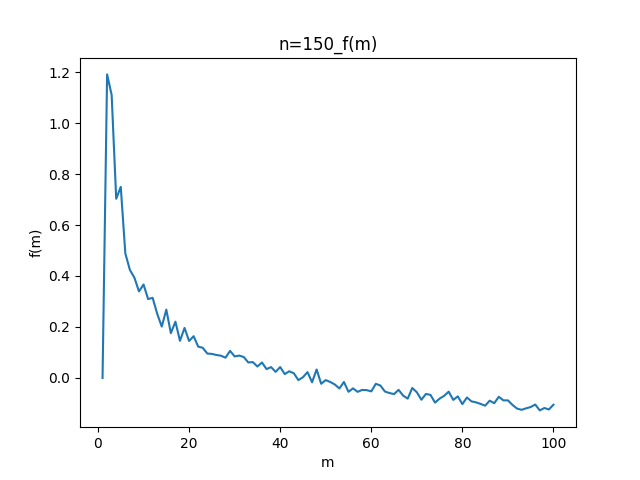
\includegraphics[height=0.25\textheight]{images/n=150_f(m).png}
    \caption{f(m) vs m for N=150}
    \label{fig:n_150_fm}
\end{figure}

\begin{figure}
    \centering
    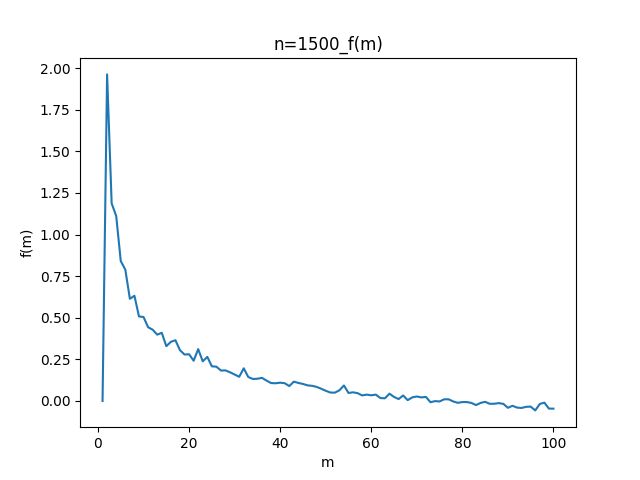
\includegraphics[height=0.25\textheight]{images/n=1500_f(m).png}
    \caption{f(m) vs m for N=1500}
    \label{fig:n_1500_fm}
\end{figure}

\begin{figure}
    \centering
    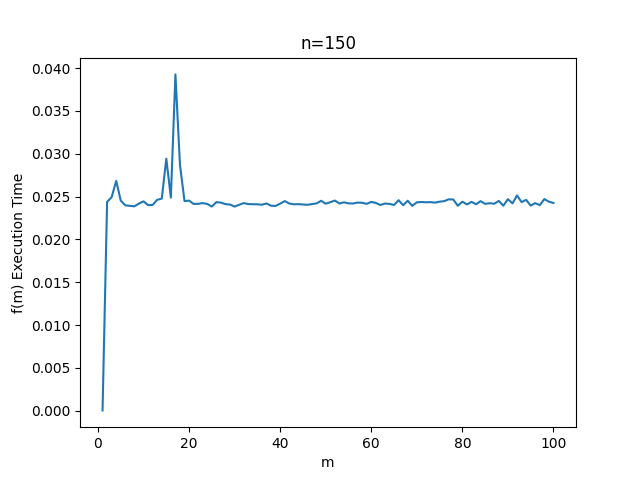
\includegraphics[height=0.25\textheight]{images/n=150.png}
    \caption{f(m) Execution Time vs m for N=150}
    \label{fig:n_150_fm_exec}
\end{figure}

\begin{figure}
    \centering
    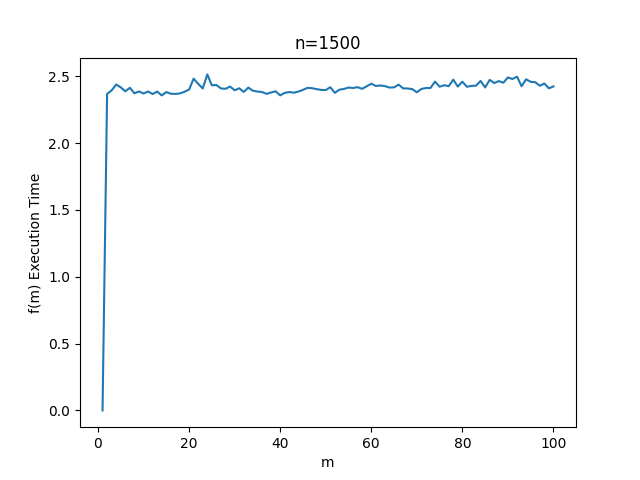
\includegraphics[height=0.25\textheight]{images/n=1500.png}
    \caption{f(m) Execution Time vs m for N=1500}
    \label{fig:n_1500_fm_exec}
\end{figure}

\begin{figure}
    \centering
    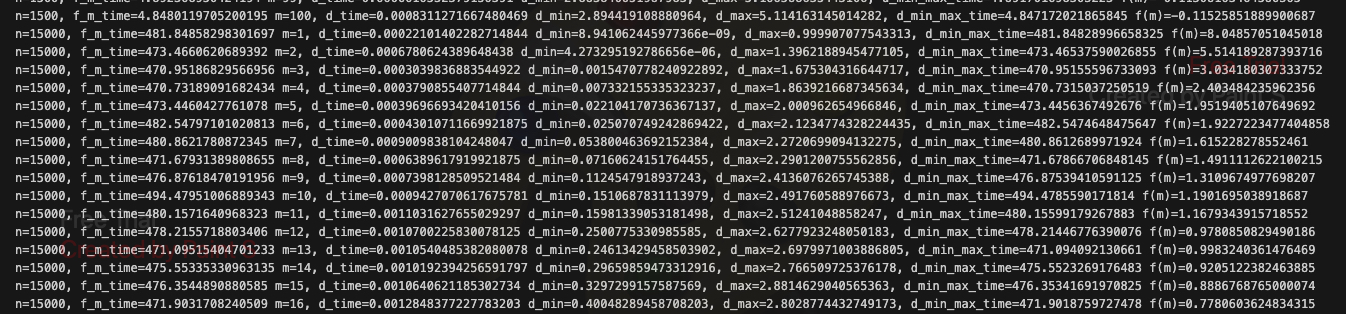
\includegraphics[width=1\textwidth]{images/jn1_timestamp.jpg}
    \caption{Curse of Dimensionality Notebook Execution Logs}
    \label{fig:cod_exectimes}
\end{figure}

\end{homeworkProblem}



%----------------------------------------------------------------------------------------
%	PROBLEM 3
%----------------------------------------------------------------------------------------

\begin{homeworkProblem}
For the following data, give the best taxonomic type (interval, ratio, nominal, ordinal):

\begin{enumerate}
 \item A section of highway on a map. - nominal 
\item The value of a stock. - ratio 
\item Your grade in the class. - ordinal 
\item Reviewing something, \textit{e.g.}, movie, purchase, food. - ordinal 
\item The weight of a person. - ratio 
\item Visiting United Airlines (https://www.united.com) the seating is: Economy,
Economy plus,
and United Business. - Nominal

\end{enumerate}

\end{homeworkProblem}

%----------------------------------------------------------------------------------------
%	PROBLEM 4
%----------------------------------------------------------------------------------------

\begin{homeworkProblem}
You are datamining with a column that includes a physical address in a  city with only one zipcode.  For example,
\begin{verbatim}

55 WEST CIR
2131 South Creek Road
Apt. #1 Fountain Park
1114 Rosewood Cir
1114 Rosewood Ct.
1114 Rosewood Drive

\end{verbatim}

What structure would you create to mine these?  What questions do you think you should be able to answer?  

\textbf{Solution}: Typically, US address follows the pattern where address line 1 contains the street address(e.g. House number, street name, etc.) and address line 2 contains the apartment number or such. The following name after that represents the city, state, and postal code. However, not necessarily this is present always and denominations after the address line 2 might not be present at all. Considering the given example we can see that the addresses presented mostly follow the address line concept mentioned before.\\

Let's number the addresses mentioned in this order for reference in our explanation,
\begin{enumerate}
    \item 55 WEST CIR
    \item 2131 South Creek Road
    \item Apt. \#1 Fountain Park
    \item 1114 Rosewood Cir
    \item 1114 Rosewood Ct.
    \item 1114 Rosewood Drive
\end{enumerate}
Now, we can see that address numbers 1,2,4,5,6 have mostly similar patterns and 3 differ at the start. From this, we can derive a brute-force method to extract the information which is, first extract the first part of an address which is most likely the house number. For example, we can number 1 can be divided into two parts 55 \& WEST CIR. We can already differentiate between area and house number. Now, for extracting information from the second part we can build a database of known street suffixes. This will help us differentiate between different streets in our addresses. Using this we can match the street address with our database remove the matched word from the street and categorize that as a street suffix. Now, the only difference here we can see is number 3 which doesn't have any street address and instead of the house number, contains the apartment number. In such cases, we can run a checker to see if an address doesn't start with a number(assuming the case is repetitive in many instances in the dataset) and have a different classifier that extracts information from this type of data. So, in general, we can project our data mining method in figure \ref{fig:address_extractor}.

\begin{figure}[h]
    \centering
    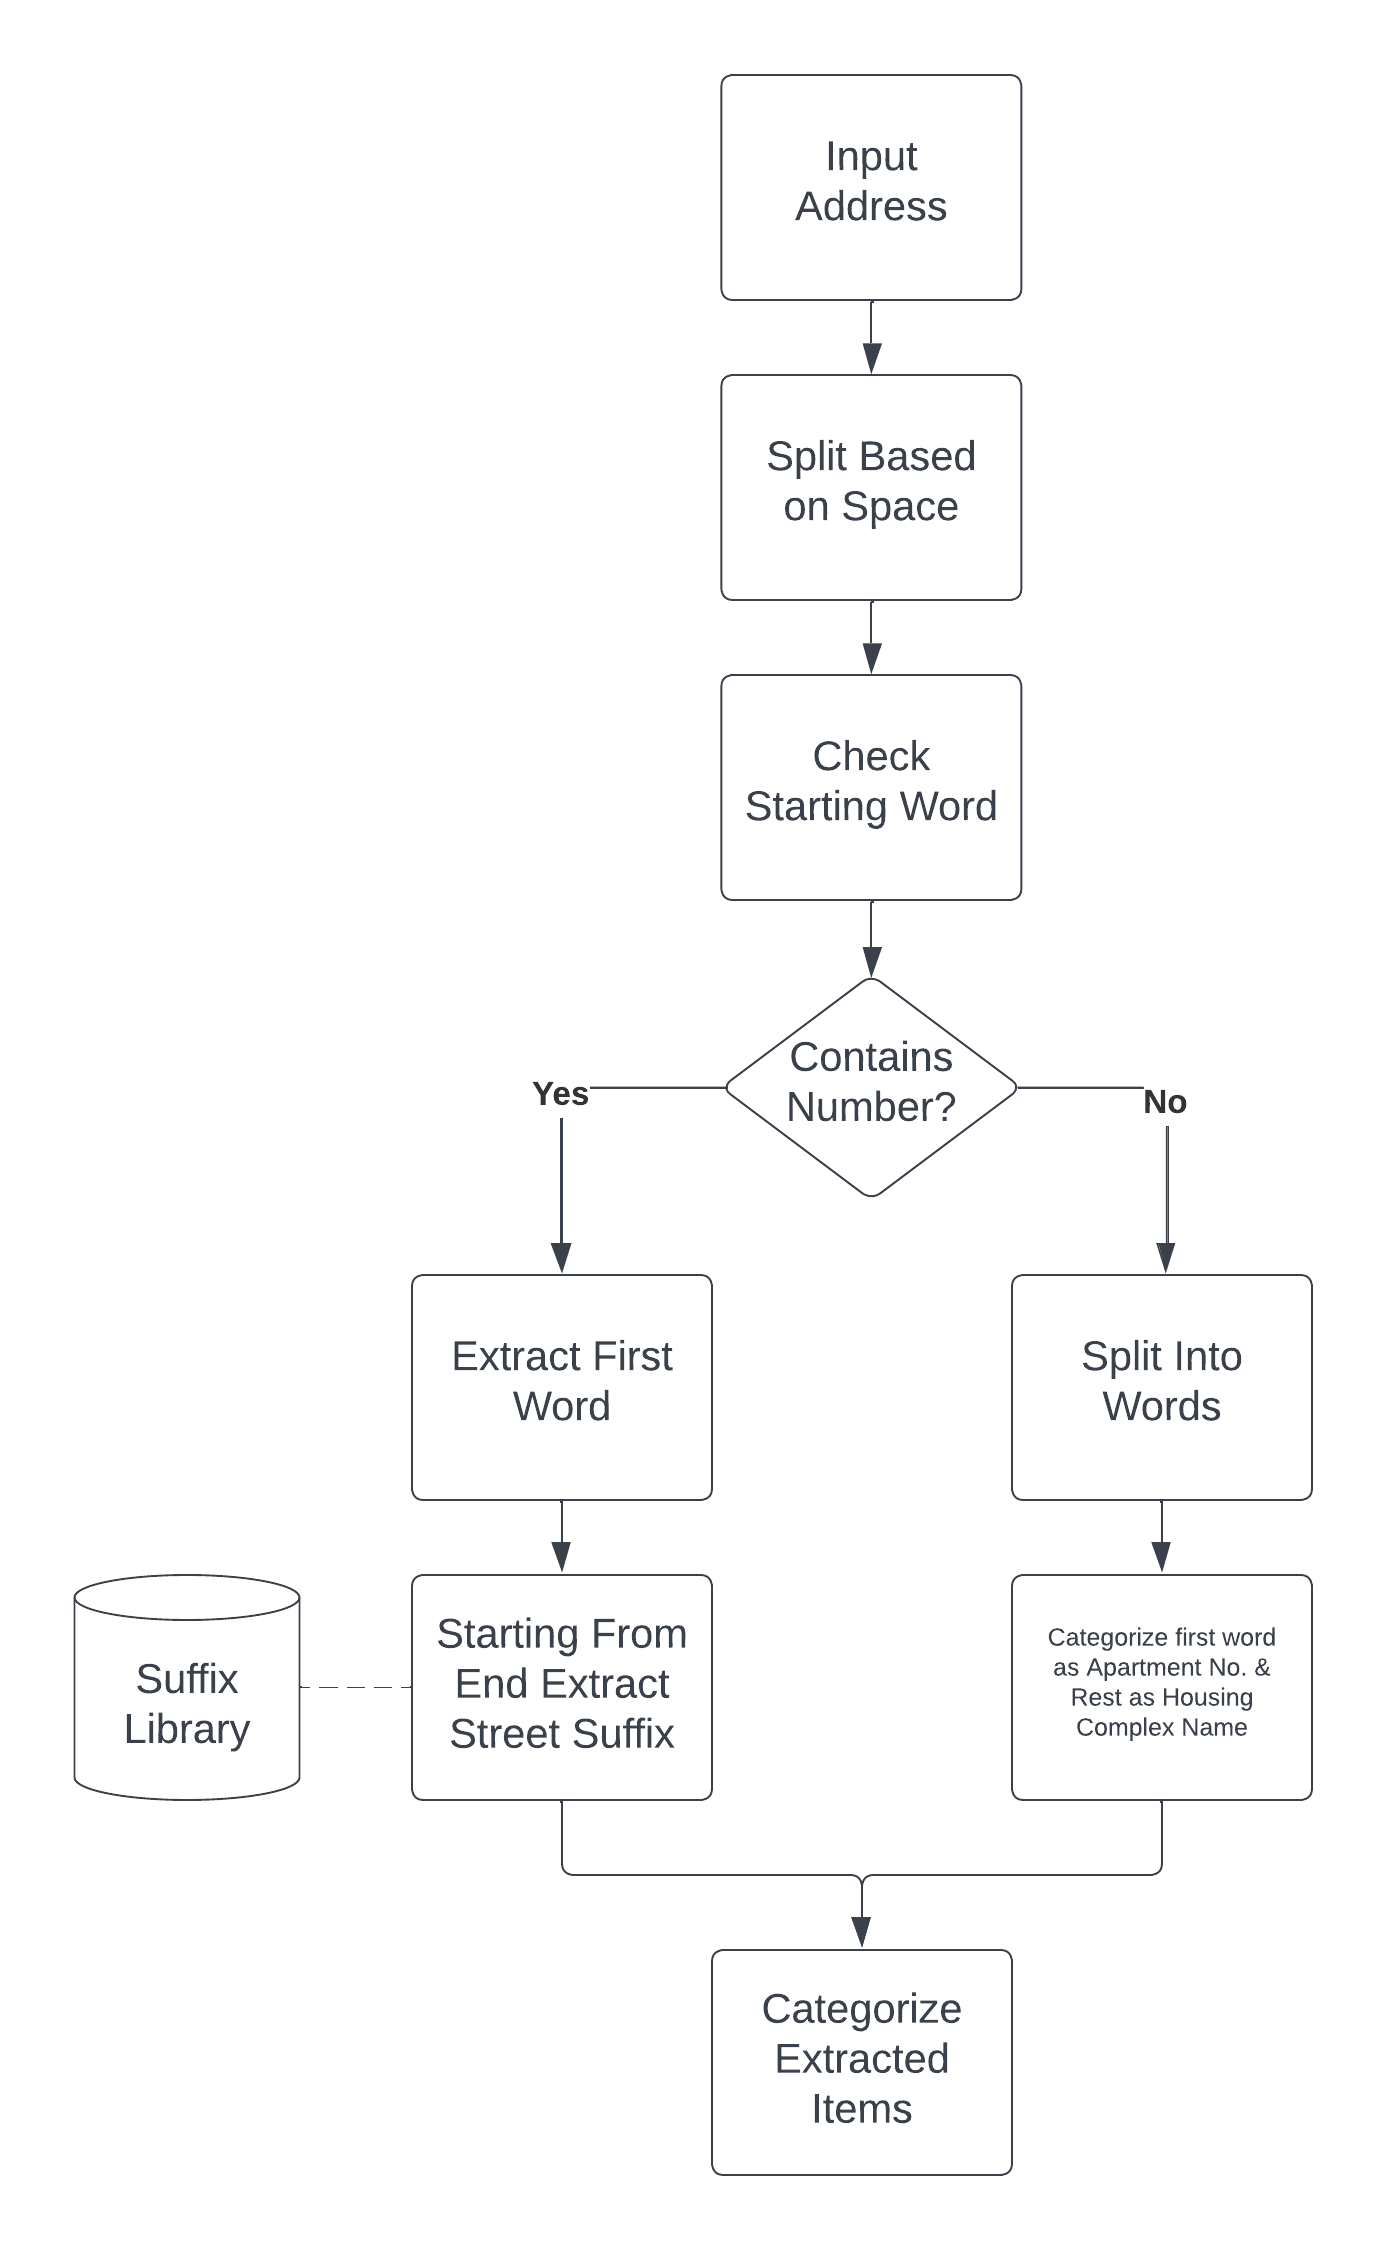
\includegraphics[width=0.5\textwidth]{images/Address Extractor Flow.png}
    \caption{Address Extraction Pipeline}
    \label{fig:address_extractor}
\end{figure}


\end{homeworkProblem}



%----------------------------------------------------------------------------------------
%	PROBLEM 5
%----------------------------------------------------------------------------------------

\begin{homeworkProblem}
For this problem, you will be using a data set with total 81 attributes of private homes in Ames, Iowa.  You'll be provided with a schema and instance.  


\subsection*{Background}
Generally this kind of data is used to determine value of a home.  Given some home $h \in H$ from the set of homes $H$,  the property taxes are $\tau \times v(h)$ where $0 \leq \tau \leq 1$ (the tax) and $v:H\rightarrow \$\mathbb{R}_{\geq 0}$ is the value.  The county auditor decides $v$ on history and similar homes.   An owner can appeal $v$ by showing $h_1,h_2,\ldots, h_6 \in H$ where $v(h_i) < v(h)$ and $h_i \approx h$ (the homes are very similar).   
\[\]
\noindent\textbf{JN II}\\
\textbf{Data Exploration using Housing Data}
\begin{itemize}
\item Determine the size (number of tuples, attribures (or features)).
\item How many missing data exist?
\item What are the three columns with the greatest number of missing data?
\item What are the three columns with the largest number of values?
\item What are the three collumns with the greatest variance? 
\item What are the three columns with the most uniform values?
\item Find 10 \textbf{individual} attributes that seem to determine the class \texttt{SalePrice}.  For this only use  sensible plotting methods.  
\item Of the 10 attributes above, show the two that seem be the most linearly related.
\end{itemize}

\subsection*{Discussion of Home Price Data}
\begin{itemize}
\item Discuss problems with determining value if you do \textit{not} look at the column data.
\item Make a histogram/bar plot for each of those 10 attributes that best determine \texttt{SalePrice}. Discuss the distribution of values, \textit{e.g.},  uniform, skewed, normal of those attributes.  Place images of these histograms into the document.  
\item Discuss the problem of determining price (numeric function).  What would be the most likely kind of model to build?
\item In your columns, discuss missing data and two techniques: remove the tuple and replace the missing value with the mean.
\end{itemize}
\textbf{Solution}:
\begin{itemize}
    \item The dataset has a total number of 1460 entries spread into 81 columns or attributes. The first column named, "Id" is more like a key for each of the instances and cannot be considered as an attribute for data analysis. So we have considered the rest of 80 attributes in our analysis. A sample of the data can be seen in figure \ref{fig:housing_sample}
    \item There are a total of 19 attributes that have missing data inside. The frequency of missing data in each attribute is projected in figure \ref{fig:missing_data}.
    \item From figure \ref{fig:missing_data} we can see that the top three attributes in terms of empty data are ``PoolQC", ``MiscFeature", and ``Alley".
    \item The three columns that has the largest values are ``SalePrice", ``LotArea", and ``MiscVal".
    \item The three columns with the greatest variances are ``SalePrice", ``LotArea", and ``GrLivArea"
    \item The three columns with the most uniform values are ``Neighborhood", ``Exterior2nd", and ``Exterior1st"
    \item The top 10 attributes with the most correlation with SalePrice are, ``OverallQual", ``OverallCond", ``FullBath", ``BsmtFinSF1", ``BsmtFinSF2", ``BsmtUnfSF", ``1stFlrSF", ``BsmtFullBath", ``BsmtHalfBath", ``GrLivArea".
    \item Now among the correlated attributes we see that only BsmtFinSF1, BsmtUnfSF, 1stFlrSF, and GrLivArea have a normal distribution and can be seen in figure \ref{fig:BsmtFinSF1}, \ref{fig:BsmtFinSF1}, \ref{fig:1stFlrSF}, and \ref{fig:GrLivArea} respectively. The other attributes are seen in figure \ref{fig:BsmtFinSF2}, \ref{fig:BsmtFullBath}, \ref{fig:BsmtFullBath}, \ref{fig:FullBath}, \ref{fig:OverallCond}, \ref{fig:OverallQual},
    \item To determine the SalPrice it is better to use a Regression analytic approach as we can see that the price of a house cannot be partitioned into $n$-classes. So, given the attributes we can run a regressor analyzer to predict the SalePrice of the houses.
    \item The issue with a missing value that we determined is very hard to impute for this experiment. For some attributes the missing values are high in percentage so to impute the missing values per se with the mean of the existing data will make the data highly biased. Also, for the categorical attributes it is not possible to use the mean-based imputation approach, however, we determined that we can use a semi-learning approach where we predict the missing values using existing classifiers and the rest of the available data. This would somewhat solve our issue, but, a high percentage of missing data in other attributes will bias the model into the training dataset. Another option is to understand the distribution of the data and try to impute data based-on the newly found distribution.
\end{itemize}

\begin{figure}
    \begin{minipage}[b]{0.5\textwidth}
        \centering
        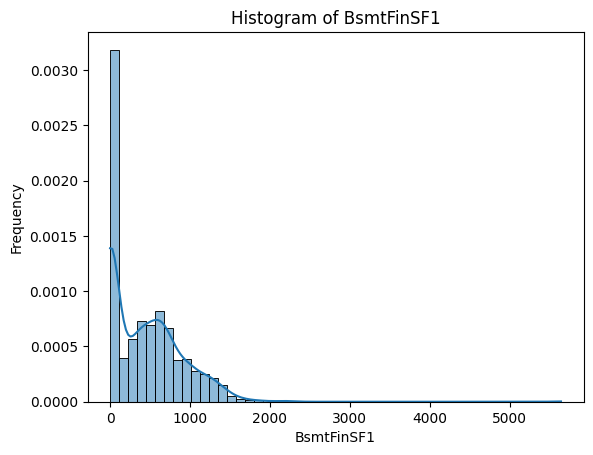
\includegraphics[width=0.9\textwidth]{images/Histogram of BsmtFinSF1.png}
        \caption{Data Distribution of BsmtFinSF1 Attribute}
        \label{fig:BsmtFinSF1}
    \end{minipage}
    \begin{minipage}[b]{0.5\textwidth}
        \centering
        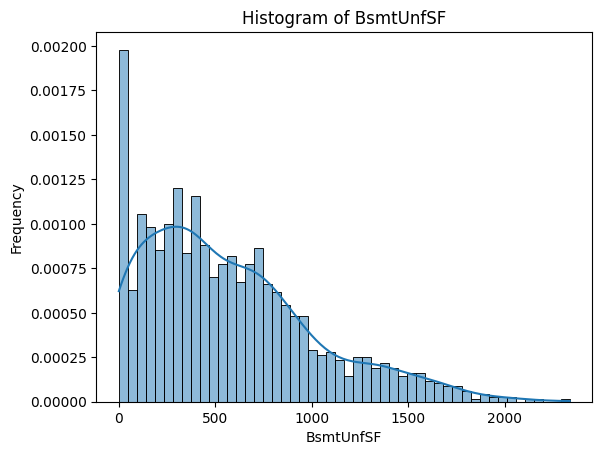
\includegraphics[width=0.9\textwidth]{images/Histogram of BsmtUnfSF.png}
        \caption{Data Distribution of BsmtUnfSF Attribute}
        \label{fig:BsmtUnfSF}
    \end{minipage}
\end{figure}

\begin{figure}
    \begin{minipage}[b]{0.5\textwidth}
        \centering
        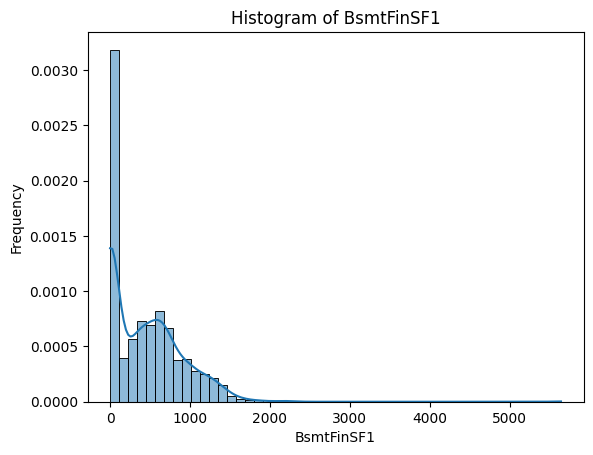
\includegraphics[width=0.9\textwidth]{images/Histogram of BsmtFinSF1.png}
        \caption{Data Distribution of BsmtFinSF1 Attribute}
        \label{fig:BsmtFinSF1}
    \end{minipage}
    \begin{minipage}[b]{0.5\textwidth}
        \centering
        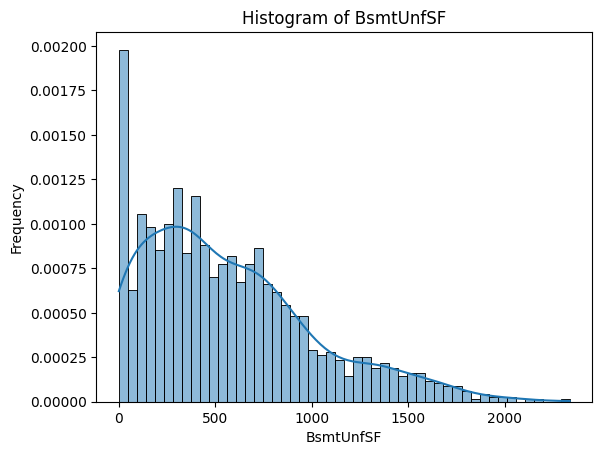
\includegraphics[width=0.9\textwidth]{images/Histogram of BsmtUnfSF.png}
        \caption{Data Distribution of BsmtUnfSF Attribute}
        \label{fig:BsmtUnfSF}
    \end{minipage}
\end{figure}

\begin{figure}
    \begin{minipage}[b]{0.5\textwidth}
        \centering
        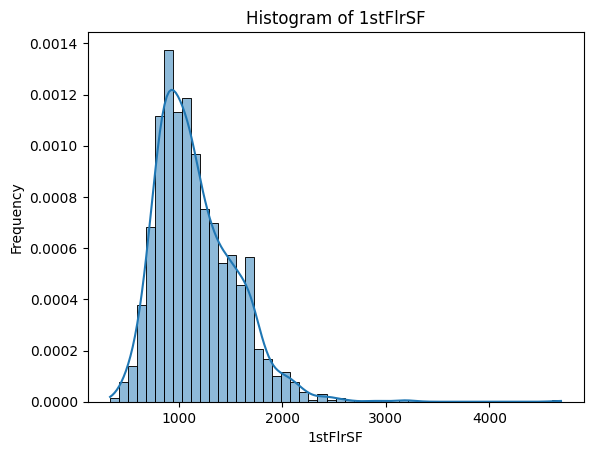
\includegraphics[width=0.9\textwidth]{images/Histogram of 1stFlrSF.png}
        \caption{Data Distribution of 1stFlrSF Attribute}
        \label{fig:1stFlrSF}
    \end{minipage}
    \begin{minipage}[b]{0.5\textwidth}
        \centering
        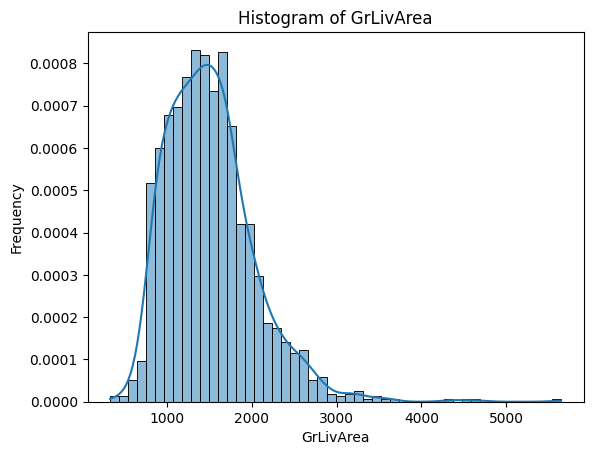
\includegraphics[width=0.9\textwidth]
    {images/Histogram of GrLivArea.png}
        \caption{Data Distribution of GrLivArea Attribute}
        \label{fig:GrLivArea}
    \end{minipage}  
\end{figure}

\begin{figure}
    \begin{minipage}[b]{0.5\textwidth}
        \centering
        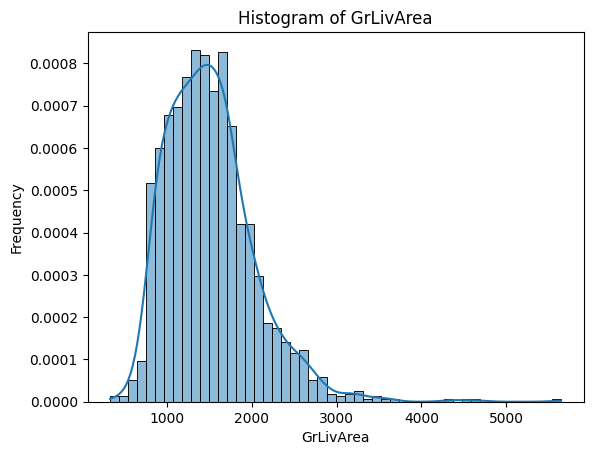
\includegraphics[width=0.9\textwidth]{images/Histogram of GrLivArea.png}
        \caption{Data Distribution of GrLivArea Attribute}
        \label{fig:GrLivArea}
    \end{minipage}
    \begin{minipage}[b]{0.5\textwidth}
        \centering
        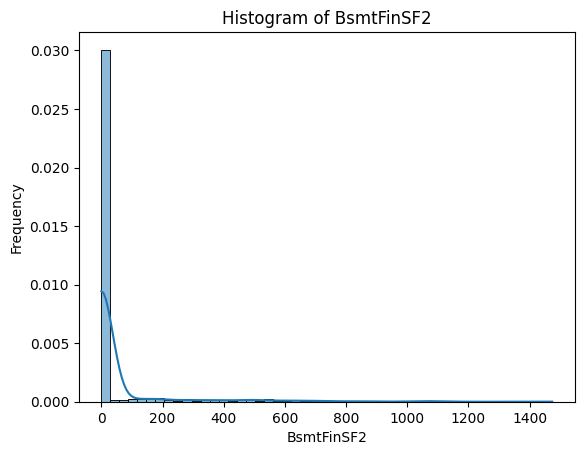
\includegraphics[width=0.9\textwidth]{images/Histogram of BsmtFinSF2.png}
        \caption{Data Distribution of BsmtFinSF2 Attribute}
        \label{fig:BsmtFinSF2}
    \end{minipage}  
\end{figure}

\begin{figure}
    \begin{minipage}[b]{0.5\textwidth}
        \centering
        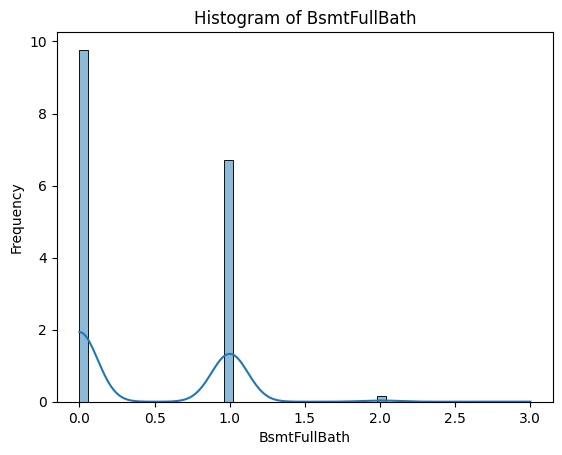
\includegraphics[width=0.9\textwidth]{images/Histogram of BsmtFullBath.png}
        \caption{Data Distribution of BsmtFullBath Attribute}
        \label{fig:BsmtFullBath}
    \end{minipage}
    \begin{minipage}[b]{0.5\textwidth}
        \centering
        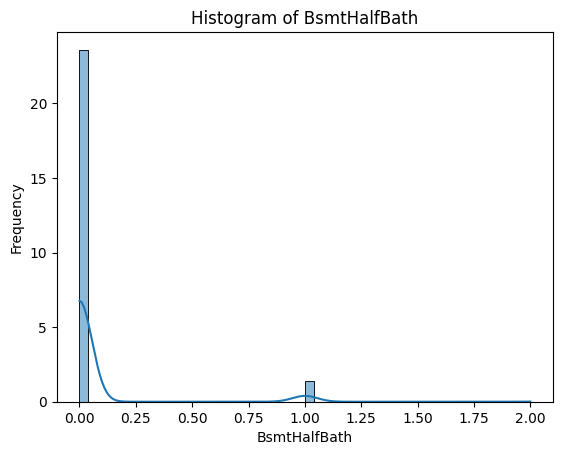
\includegraphics[width=0.9\textwidth]{images/Histogram of BsmtHalfBath.png}
        \caption{Data Distribution of BsmtHalfBath Attribute}
        \label{fig:BsmtHalfBath}
    \end{minipage}  
\end{figure}

\begin{figure}
    \begin{minipage}[b]{0.5\textwidth}
        \centering
        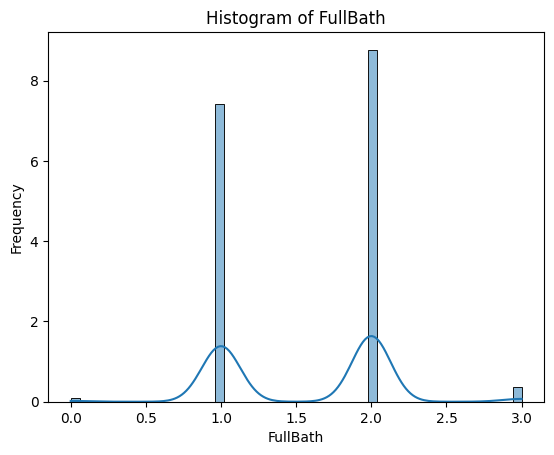
\includegraphics[width=0.9\textwidth]{images/Histogram of FullBath.png}
        \caption{Data Distribution of FullBath Attribute}
        \label{fig:FullBath}
    \end{minipage}
    \begin{minipage}[b]{0.5\textwidth}
        \centering
        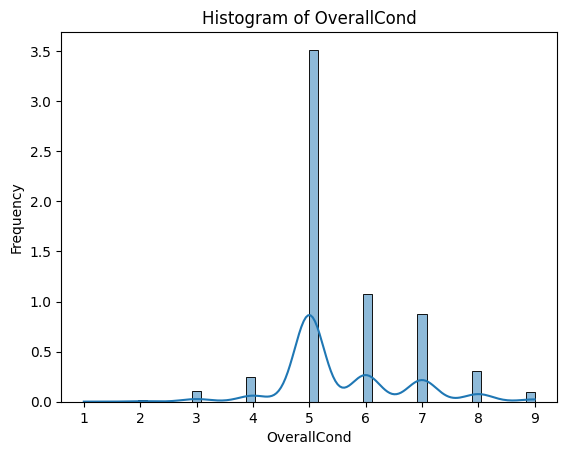
\includegraphics[width=0.9\textwidth]{images/Histogram of OverallCond.png}
        \caption{Data Distribution of OverallCond Attribute}
        \label{fig:OverallCond}
    \end{minipage}  
\end{figure}

\begin{figure}
    \centering
    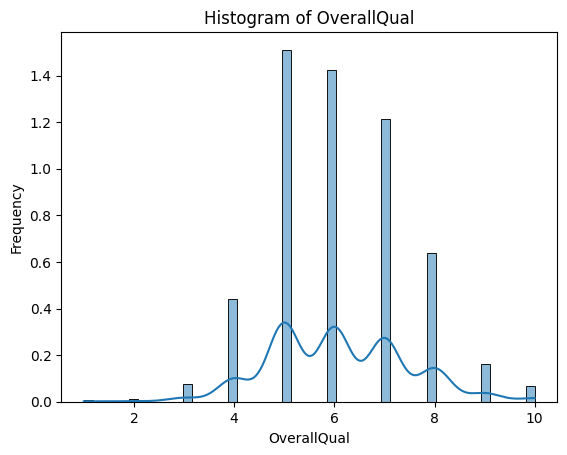
\includegraphics[width=0.5\textwidth]{images/Histogram of OverallQual.png}
    \caption{Data Distribution of OverallQual Attribute}
    \label{fig:OverallQual}
\end{figure}


\end{homeworkProblem}

\begin{figure}
    \centering
    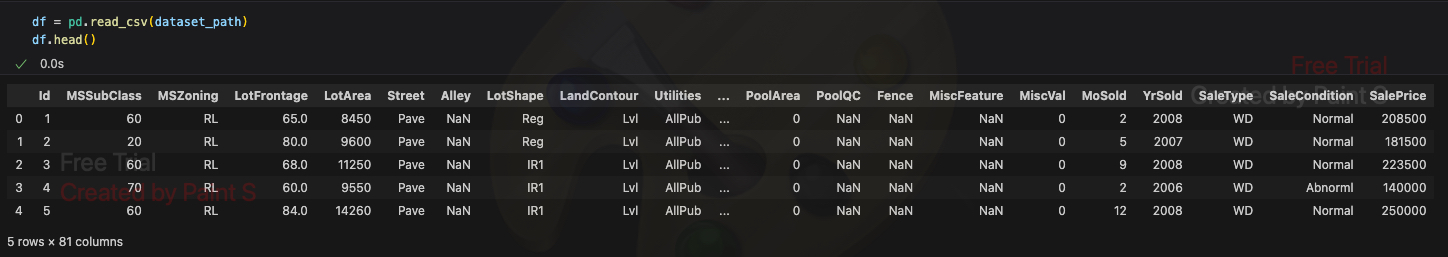
\includegraphics[width=1\textwidth]{images/housing_data_sample.jpg}
    \caption{Sample Data From Housing Dataset}
    \label{fig:housing_sample}
\end{figure}

\begin{figure}
    \centering
    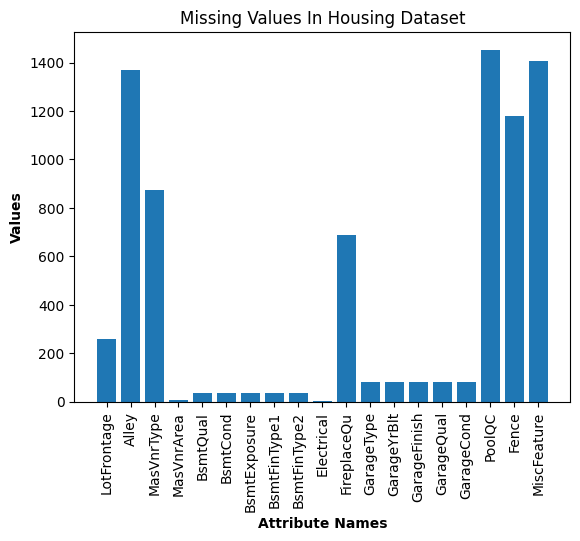
\includegraphics{images/missing_values.png}
    \caption{Number of Missing Data in the Columns of Housing Dataset}
    \label{fig:missing_data}
\end{figure}


%----------------------------------------------------------------------------------------
%	PROBLEM 6
%----------------------------------------------------------------------------------------

\begin{homeworkProblem} 


Distinguish between noise and outliers. Be sure to consider the following questions.
\begin{enumerate}
    \item Is noise ever interesting or desirable? Outliers?
    \item Can noise objects be outliers?
    \item Are noise objects always outliers?
    \item Are outliers always noise objects?
    \item Can noise make a typical value into an unusual one, or vice versa?
\end{enumerate}

\textbf{Solution}: According to \cite{Salgado2016}, the main difference between noise and outlier is that noise is most likely an input error or mislabeling whereas, outlier is not an error but rather an underrepresented region in the dataset. However, it is very easy to misrepresent noise as an outlier as both have some similar characteristics. It is better to explain this phenomenon through an example. Suppose, we have the following age data of humans represented in years, $d_{age} = [15,18,23,34,500]$ and another data, weight of vehicles, $d_{weight} = [500, 1200, 900, 10000]$ represented in \textit{kg's}. Now, for $d_{age}$, we can see that 500 is a noise as it is highly unlikely that a person's age is 500. It is possible that due to data insertion a $0$ was added mistakenly. However, if we look at the data points of $d_{weight}$ it is not entirely clear whether that is a noise or an outlier. It is mentioned the given weights are for vehicles but the type of vehicle wasn't mentioned so it is possible that although the first few data points refer to family cars, the last one might be an industrial vehicle. Another possibility is, of course, this data being a noise which was an error while input. So, depending on the context a datapoint that is not consistent with the dataset might or might not be an outlier or vice versa. However, noise can be easily identified if for example, our $d_{age}$ contained a value such as ``New York City". Here it is evident that this is a string and essentially the name of a city, hence, it is a noise. Apart from the scenario just mentioned for the noise, both noise and outlier can create significant issues while analysing the data. As it will skew the dataset remarkably and will affect pattern recognition tasks. With the increase in noise and/or outliers, the distribution of data becomes unstable. So, in short, although both of them contain similarities and dissimilarities, the presence of either can affect the understanding of the data on a huge scale.


\end{homeworkProblem}

%----------------------------------------------------------------------------------------
%	PROBLEM 7
%----------------------------------------------------------------------------------------

\begin{homeworkProblem} 
Assume you have data $D = \{x_0, x_1,x_2,x_3\}$.  Provide a listing of all the possible partitions.\\
\textbf{Solution}: Using bells triangle\cite{btriangle} we find the number of partitions to be 15 as listed below

\begin{enumerate}
    \item Partition 1: \( \{\{x_0, x_1, x_2, x_3\}\} \)
    \item Partition 2: \( \{\{x_0\}, \{x_1, x_2, x_3\}\} \)
    \item Partition 3: \( \{\{x_1\}, \{x_0, x_2, x_3\}\} \)
    \item Partition 4: \( \{\{x_2\}, \{x_0, x_1, x_3\}\} \)
    \item Partition 5: \( \{\{x_3\}, \{x_0, x_1, x_2\}\} \)
    \item Partition 6: \( \{\{x_0, x_1\}, \{x_2, x_3\}\} \)
    \item Partition 7: \( \{\{x_0, x_2\}, \{x_1, x_3\}\} \)
    \item Partition 8: \( \{\{x_0, x_3\}, \{x_1, x_2\}\} \)
    \item Partition 9: \( \{\{x_0\}, \{x_1\}, \{x_2, x_3\}\} \)
    \item Partition 10: \( \{\{x_0\}, \{x_2\}, \{x_1, x_3\}\} \)
    \item Partition 11: \( \{\{x_0\}, \{x_3\}, \{x_1, x_2\}\} \)
    \item Partition 12: \( \{\{x_1\}, \{x_2\}, \{x_0, x_3\}\} \)
    \item Partition 13: \( \{\{x_1\}, \{x_3\}, \{x_0, x_2\}\} \)
    \item Partition 14: \( \{\{x_2\}, \{x_3\}, \{x_0, x_1\}\} \)
    \item Partition 15: \( \{\{x_0\}, \{x_1\}, \{x_2\}, \{x_3\}\} \)
\end{enumerate}


\end{homeworkProblem}

%----------------------------------------------------------------------------------------
%	PROBLEM 8
%----------------------------------------------------------------------------------------

\begin{homeworkProblem}
Consider a document-term matrix, where $tf_{ij}$ is the frequency of the $i^{th}$ word (term) in the $j^{th}$ document and $m$ is the number of documents. Consider the variable transformation that is defined by
$$tf^{'}_{ij} = tf_{ij} \times \log\frac{m}{df_{i}},$$
where $df_{i}$ is the number of documents in which the $i^{th}$ term appears, which is known as the document frequency of the term. This transformation is known as inverse document frequency transformation.
\begin{enumerate}
    \item What is the effect of this transformation if a term occurs in one document? In every document?
    \item What might be the purpose of this transformation?
\end{enumerate}
\textbf{Solution}: The inverse document frequency transformation, also known as $tf-idf$ transformation is a technique we used to find the effectness of a word in a document\cite{tfidf}. The given equation describes a lot about how the term can be affected in a document. For instance, we can see that given $m$-documents and several occurrences of a term $df_i$, the transformation is proportionate to its logarithmic value. Now, as a term occurs in just one document the effect of this transformation will be higher. However, as the term appears more and more in the document the effect lessens and goes to 0. This is ensured by the high term frequency and low document frequency in the entirety of the $m$-documents.
\end{homeworkProblem}

%----------------------------------------------------------------------------------------
%	PROBLEM 9
%----------------------------------------------------------------------------------------

\begin{homeworkProblem}
This question compares and contrasts some dissimilarity measures.
\begin{enumerate}
    \item For binary data, the L1 distance corresponds to the Hamming distance; that is, the number of bits that are different between two binary vectors. The Jaccard similarity is a measure of the similarity between two binary vectors. Compute the Hamming distance and the Jaccard similarity between the following two binary vectors.\\
    \begin{itemize}
        \item $\textbf{x} = 0101010001$
        \item $\textbf{y} = 0100011000$
    \end{itemize}
        \textbf{Solution}: Given, $x=0101010001$ and $y=0100011000$Now the Hamming distance of $x$ and $y$ is, $3$ as there are 3 different elements while going through both of the arrays sequentially.\\
        The Jaccard similarity is defined by the formula\cite{jaccard},
        \begin{equation}
            J(A,B) = \dfrac{A \cap B}{A \cup B}
        \end{equation}
        Where $A$,$B$ denotes two vectors, $A \cup B$ denotes the total number of points between both of the vectors, and $A \cap B$ denotes the similar vector between them. So for Jaccard similarity we get, $x \cap y = 3$ and  $x \cup y = 17$.\\
        Thus, $J(x,y)=3/17=0.176$. \\
    \item Which approach, Jaccard or Hamming distance, is more similar to the Simple Matching Coefficient, and which approach is more similar to the cosine measure? Explain. (Note: The Hamming distance is a distance, while the other three measures are similar, but don't let this confuse you.)\\
        \textbf{Solution}: Simple Matching Coefficient(SMC), also known as Rand Similarity Coefficient generally serves as a similarity and diversity comparison method\cite{smc}. This is very similar to the Jaccard similarity coefficient as the method of finding the similarity in SMC follows the same pattern as Jaccards in finding the ratio of the total matched vector and the total number of vectors present.
    \item Suppose that you are comparing how similar two organisms of different species are in terms of the number of genes they share. Describe which measure, Hamming or Jaccard, you think would be more appropriate for comparing the genetic makeup of two organisms. Explain. (Note: Assume that each animal is represented as a binary vector, where each attribute is $1$ if a particular gene is present in the organism and $0$ otherwise.)\\
        \textbf{Solution}: Finding the most similar between two species accounts for a lot of questions. First of all, if we are comparing two species that belong to the same genre then it is likely that they share a lot of characteristics. An article\cite{genome} addresses how similar the species are because of the shared ancestors in the species tree. So, to efficiently find cross-species similarity it is better to use ``Jaccard Similarity" instead of ``Hamming Distance" as the former considers the shared genes as well as dissimilar genes. For example, let two species $S_1$ and $S_2$ have 1 similar gene and they contain a total of 2 genes (Assumption for the simplicity of the example). Now the ``Hamming" distance would simply say that they have a distance of just 1, from which we might assume that they are not that similar. On the other hand, ``Jaccard" similarity would consider the total number of genes and would result in saying that $S_1$ and $S_2$ are very similar. It can be further argued by extending the total number of genes between the species.
    \item If you wanted to compare the genetic makeup of two organisms of the same species, e.g., two human beings, would you use the Hamming distance, the Jaccard
    coefficient, or a different measure of similarity or distance? Explain. (Note: Two human beings share $> 99.9\%$ of the same genes.)\\
    \textbf{Solution}: Sequence Alignment\cite{sequenceAlignment} is a popular method in bioinformatics to compare genetic similarity. We would prefer this method over the Jaccard similarity and Hamming distance because of the following reasons,
    \begin{itemize}
        \item Dynamic Programming Solution so makes the calculation faster
        \item Can easily handle different length sequences
        \item Considers not only the similarities but also the substitutions of genomes
        \item Can capture more semantics
    \end{itemize}
\end{enumerate}
\end{homeworkProblem}
%----------------------------------------------------------------------------------------
%	PROBLEM 10
%----------------------------------------------------------------------------------------

\begin{homeworkProblem}
\noindent\textbf{JN III}\\
For the following vectors, $\textbf{x}$ and $\textbf{y}$, calculate the indicated similarity and distance measures. Show detailed calculations/steps.
\textbf{Solution:} The result and calculations and Python implementation can be found for this problem in the file \textit{jn3.ipynb}. The formula for Cosine, Correlation, Jaccard, and Euclidean is adapted from various sources\cite{cSimilarity} \cite{pearson} \cite{jaccard} \cite{euclidean}. Kindly note that for correlations, we have used ``Pearson's Correlation Coefficient" to find the correlations.
\begin{enumerate}
    \item $\textbf{x} = (1,1,1,1)$, $\textbf{y} = (2,2,2,2)$ cosine, correlation, Euclidean.\\
    \textbf{Solution}: The cosine similarity of the vectors was found to be 1. Looking at the vector we can see that each of the elements in the vector is differed by just 1. Now, given the definition of cosine similarity, the result represents that the angle between the vectors is low. This denotes that the vectors are very similar. For correlation calculations, as the vectors don't have any variance in the Pearson's method is not able to calculate any correlations between them. Since correlations are calculated based on deviation and the deviations of the vectors are 0 a calculation is not possible. The result for Euclidean distance was found to be 2.
    \item $\textbf{x} = (0,1,0,1)$, $\textbf{y} = (1,0,1,0)$ cosine, correlation, Euclidean, Jaccard.\\
    \textbf{Solution}: The results for cosine, correlation, Jaccard, and Euclidean distance were found to be 0, -1, 2, 0. Looking at the vectors we can easily understand the results here. First of all, we can see that element-wise the vectors differ on every element. Thus, there is no similarity between them. Second of all, due to the difference in each unit, the correlation is -1. Last of all, the Euclidean distance we find is similar to \textit{Problem a} but from the similarity index, we can determine that the vectors are not similar.
    \item $\textbf{x} = (0,-1,0,1)$, $\textbf{y} = (1,0,-1,0)$ cosine, correlation, Euclidean.\\
    \textbf{Solution}: Interestingly here, the results are 0 for cosine similarity, 0 for correlation, and 2 for distance. We can understand the result being 0 for similarity as the vectors differ by elements, however, the correlation being 0 changes the fact that we received -1 for the previous problem. Due to the nature of variance, we argue that the correlation achieved a different result. Finally, the distance seems to be unchanged given the variance has changed.
    \item $\textbf{x} = (1,1,0,1,0,1)$, $\textbf{y} = (1,1,1,0,0,1)$ cosine, correlation, Jaccard.\\
    \textbf{Solution}: For this problem, we see a slight difference in similarity for Jaccard and cosine similarity which is 0.5 and 0.75 respectively. Looking at the vectors and how Jaccard and cosine similarity is defined we argue that due to the nature of Jaccard's similarity of eliminating common elements between vectors, it generates lower similarity results than the other one. The correlations are again determined by the variance of the dataset and in this case the vectors.
    \item $\textbf{x} = (2,-1,0,2,0,-3)$, $\textbf{y} = (-1,1,-1,0,0-1)$ cosine, correlation.\\
    \textbf{Solution}: Due to the different valued elements in the vectors, we see a similarity score of 0 for this problem. For correlation, the value seems to be very low which again certifies the similarity factor.
\end{enumerate}
\end{homeworkProblem}


\printbibliography
\end{document}